\chapter{Python\index{Python}}
\thispagestyle{fancy}
\lstset{}\lstset{language=Python, style=pythonstyle}

Python is a high-level, interpreted programming language known for its simplicity, readability, and versatility. With its elegant syntax and dynamic typing, Python facilitates rapid development and prototyping across various domains, including web development, data analysis, artificial intelligence, and scientific computing. Its extensive standard library and vibrant ecosystem of third-party packages provide comprehensive support for a wide range of tasks, from basic scripting to complex software development. Python's object-oriented and functional programming paradigms, coupled with its strong community support and cross-platform compatibility, make it an ideal choice for both beginners and experienced developers seeking efficient and expressive solutions to their programming challenges. Its emphasis on code readability and simplicity distinguishes Python from other languages, promoting maintainability and collaboration in software projects.

\myindent The official python documentation can be found at the following links
\begin{lstlisting}
# Documentation for version 3+
https://docs.python.org/3/
# Documentation for version 2+
https://docs.python.org/2/
\end{lstlisting}











\section{Basics of Python}












\subsection{Imports and libraries}

Import floating point division which allows python 2 compatibility when using division with doubles. Include this at the beginning of the script.
\begin{lstlisting}
from __future__ import division
\end{lstlisting}

On Linux, there's a site-packages folder that imported libraries are all in. These are located in the following directories for python versions 2.7 and 3.6 respectively.

\begin{itemize}
	\item /usr/lib/python2.7/site-packages
	\item /usr/lib/python3.6/site-packages
\end{itemize}

I believe you only have specify the path from that folder on. For example, an app that uses the import program.script.interface as interface will have the interface.py file installed to usr/lib/python3.6/site-packages/program/scripts.









\subsection{Program parameters}

You can add input parameters for a python script/program using the argparse package.
\begin{lstlisting}
import argparse

parser.add_argument(
		'-v',							# Creats a parameter with -v
		'--verbose',					# Creates args.verbose parameter
		required=False,					# Sets the parameter to not required.
		default=False,					# Sets default value
		action='store_true',			# Sets value to true if supplied
		help="Enables verbose mode.")	# Sets help message
					
parser.add_argument(
		'-i',							# Creates a parameter with -i
		'--input',						# Creates args.input parameter
		required=True,					# Sets the parameter to be required
		default="potato",				# Sets default value to "potato"
		help="An input string to use")	# Sets a help message
		
if args.input is not none:
	print("Input value is {0}".format(args.input)) # prints the input value.
	
if args.verbose:
	print("Verbose is on!")
\end{lstlisting}





\subsection{Methods, Functions, and Classes}


To define a \idx{function} in Python, you use the \idx{def} keyword followed by the function name and parameters, if any. You can also include a docstring to provide documentation for the function. In this example, the \texttt{greet}() function takes a \texttt{name} parameter and returns a greeting message.
\begin{lstlisting}
def greet(name):
    """
    This function greets the user.
    :param name: The name of the person to greet
    :return: A greeting message
    """
    return f"Hello, {name}!"
\end{lstlisting}


\idx{Methods} are functions that are associated with objects. They are defined within the scope of a class and are accessed through instances of the class. In this example, the \texttt{bark}() method of the \texttt{Dog} class prints a bark message when called.
\begin{lstlisting}
class Dog:
    def bark(self):
        """
        This method makes the dog bark.
        """
        print("Woof!")
\end{lstlisting}

\idx{Classes} in Python allow you to define your own data types with custom attributes and methods. In this example, the \texttt{Rectangle} class represents a geometric rectangle. It has an \idx{\_\_init\_\_}() method to initialize its width and height attributes and an \texttt{area}() method to calculate its area.
\begin{lstlisting}
class Rectangle:
    def __init__(self, width, height):
        self.width = width
        self.height = height
        
    def area(self):
        return self.width * self.height
\end{lstlisting}

To use the \texttt{Rectangle} class, you can create an instance of it by passing the width and height values as parameters to the constructor:
\begin{lstlisting}
# Constructing a Rectangle object
rectangle1 = Rectangle(5, 10)

# Calculating the area of the rectangle
area = rectangle1.area()

print("The area of the rectangle is:", area)
\end{lstlisting}








\subsection{String manipulation}

To split a string by a \idx{delimiter} you can use the \idx{split}() method. To remove any leadig or trailing \idx{whitespace} from a string, you can use the \idx{strip}() method. Additionally, you can use \idx{lstrip}() to remove leading whitespace and \idx{rstrip}() to remove trailing whitespace.
\begin{lstlisting}
stringValue = "Test; string "

firstPart = stringValue.split(';')[0] 	# Stores "Test"
secondPart = stringValue.split(';')[1]	# Stores " string "
noWhiteSpace = secondPart.strip()       # Stores "string"
leftWhiteSpace = secondPart.lstrip()    # Stores "string "
rightWhiteSpace = secondPart.rstrip()   # Stores " string"
\end{lstlisting}

The opposite of splitting strings is joining them. You can use the \idx{join}() method to concatenate a sequence of strings into a single string, using a specified delimiter.
\begin{lstlisting}
words = ['Hello', 'world', '!']

# Join the words with a space delimiter
sentence = ' '.join(words)   # Stores "Hello world !"
\end{lstlisting}

Python provides methods to convert the case of strings. You can use \idx{lower}() to convert a string to lowercase and \idx{upper}() to convert it to uppercase.

\begin{lstlisting}
text = "Hello, World!"

# Convert the string to lowercase
lowerCaseText = text.lower()   # Stores "hello, world!"

# Convert the string to uppercase
upperCaseText = text.upper()   # Stores "HELLO, WORLD!"
\end{lstlisting}

To insert variables into a string, you can use the \idx{format}() method or by using an \idx{f-string} (introduced in python3.6).
\begin{lstlisting}
a = 5
b = 6
sum = a + b
equation = "{0} + {1} = {2}".format(a, b, sum)
f_equation = f"{a} + {b} = {sum}"

print(equation)   # prints "5 + 6 = 11"
print(f_equation) # prints "5 + 6 = 11"
\end{lstlisting}









\subsection{Arrays and lists}

To check if any value in one array or list is present in another array or list, you can use the \idx{any}() function along with a generator expression. In this example, the \idx{any}() function iterates over each item in \texttt{list2} and checks if it is present in \texttt{list1}. If any common elements are found, the condition evaluates to \texttt{True}, and the corresponding message is printed.
\begin{lstlisting}
list1 = ["apple", "banana", "orange"]
list2 = ["orange", "grape", "pear"]

if any(item in list1 for item in list2):
    print("Common elements found between list1 and list2")
else:
    print("No common elements found")
\end{lstlisting}
 
You can concatenate two or more lists using the \idx{+ operator} or the \idx{extend}() method. Both methods produce the same result: a new list containing all the elements from the original lists in the specified order.
\begin{lstlisting}
list1 = [1, 2, 3]
list2 = [4, 5, 6]

# Using the + operator
concatenated_list = list1 + list2   # Stores [1, 2, 3, 4, 5, 6]

# Using the extend() method
list1.extend(list2)   # Modifies list1 to [1, 2, 3, 4, 5, 6]
\end{lstlisting}

To find the number of elements in a list, you can use the built-in \idx{len}() function.
\begin{lstlisting}
my_list = [10, 20, 30, 40, 50]

# Find the length of the list
list_length = len(my_list)   # Stores 5
\end{lstlisting}








\subsection{Plotting and Graphs\index{Plotting and Graphs}}

A nicely formatted plot with a legend using the pylab package.
\begin{lstlisting}
import pylab as plt #Imports the correct packages for plotting.

plt.title('Contamination & Beam Health % vs Time')      # Creates a title.

plt.plot(t, Contamination, '-b', label='Contamination') # Plots Contamination in blue.
plt.plot(t, Beam_loss, '-r', label='Beam Loss')     # Plots Beam_loss in red.
plt.plot(t, Beam_health, '-g', label='Beam Health') # Plots Beam_health in green.

plt.xlabel("time (seconds)")   # Creates a x-axis label
plt.ylabel("Contamination %")  # Creates a y-axis label

plt.legend(loc='center right') # Creates a legend with the labels set above.
# Other locations include upper/lower/center left/right

plt.show() # Displays plot.
\end{lstlisting}
This code would display a graph such as the one below such that the proper values are input.

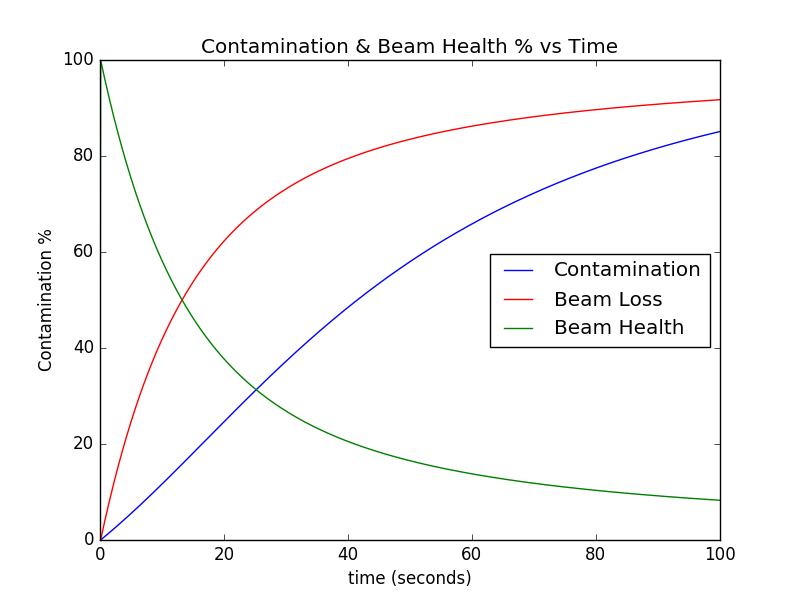
\includegraphics[width=0.5\linewidth]{./Images/Figures/figure_1-4}

A nicely formatted plot with a legend using the matplotlib package.
\begin{lstlisting}
import matplotlib as plt    # Imports the correct packages for plotting.

fig = plt.figure(dpi=1200)  # Increase resolution of the plot.
plt.scatter(x, y, s=0.1)    # Plot x data vs y data with a dot size of 0.1.
fig.suptitle(title, fontsize=12) # adds a title to the figure.

plt.xlabel("x axis label")  # Creates a x-axis label.
plt.ylabel("y axis label")  # Creates a y-axis label.

manage = plt.get_current_fig_manager()
manage.full_screen_toggle() # Makes the plt full screen.

plt.show()                  # Displays plot.
plt.savefig("fileName.png") # Saves the figure as an image
\end{lstlisting}





























\section{Pytest \index{Pytest}}

\idx{Pytest} is a powerful and popular testing framework for Python that simplifies the process of writing and executing tests. It offers a straightforward syntax and extensive features for writing test cases, including assertions, fixtures, parameterization, and test discovery. Pytest provides robust support for testing different types of applications, including web applications, APIs, and command-line utilities. It promotes efficient testing practices by emphasizing readability, scalability, and flexibility, making it a preferred choice for many Python developers.

\myindent To run a python test file using pytest, you can call pytest directly via a terminal.
\begin{lstlisting}
pytest -vv test_my_module.py
\end{lstlisting}

To write tests for a function, you must import that function and write a test for it. The \idx{assert} is a basic test keyword is used to check if a statement is true of false.
\begin{lstlisting}
# Code implementation in a Python file (e.g., my_module.py)

def add(x, y):
    """Function to add two numbers."""
    return x + y
\end{lstlisting}

\begin{lstlisting}
# Test case using Pytest (e.g., test_my_module.py)

import pytest
import my_module

def test_add():
    """Test case for the add function."""

    # Test with positive integers
    assert my_module.add(2, 3) == 5
    
    # Test with negative integers
    assert my_module.add(-2, -3) == -5
    
    # Test with zero
    assert my_module.add(0, 0) == 0
    
    # Test with one positive and one negative integer
    assert my_module.add(5, -3) == 2
\end{lstlisting}

A pytest \idx{fixture} can be used to create a \idx{temporary directory} for testing.

\begin{lstlisting}
import pytest

@pytest.fixture
def temp_directory():
    """
    Fixture to create a temporary directory for testing.

    This fixture creates a temporary directory using tempfile.mkdtemp().
    The temporary directory path is provided to the test functions, and after testing,
    the temporary directory is removed to clean up resources.

    Yields:
        str: Path of the temporary directory.
    """
    # Create a temporary directory for testing
    temp_dir = tempfile.mkdtemp()
    # Provide the temporary directory to the test for its duration.
    yield temp_dir

# Call a method using the temp_directory() method.
def test_method(temp_directory):
	print(temp_directory) # Prints the temp directory path
\end{lstlisting}

A pytest \idx{fixture} can be used to return an instance of a class.

\begin{lstlisting}
import pytest
from mmorpdnd import MMORPDND

@pytest.fixture
def mmorpdnd_instance():
    """
    Fixture to provide an instance of the MMORPDND class for testing.
    """
    return MMORPDND()
\end{lstlisting}

You can define a list of test \idx{parameters} to be input into a test via the \idx{@pytest.mark.parametrize} decorator, allowing multiple input-output pairs to be tested with the same test function.

\begin{lstlisting}
@pytest.mark.parametrize("input_string, expected_output", [
    ("'6 (barbarian 3, rogue 3)'", 6),
    ("'12 dwarfs and 3 elves'", 12),
    ("'No numbers here!'", None),
    ("'Only one number: 42'", 42),
    ("'Negative number: -10'", -10),
    ("'Integers: 1 2 3'", 1),
    ("'999'", 999),
])
def test_extract_first_integer(input_string, expected_output):
    """
    Test case to verify the behavior of extract_first_integer function.
    """
    assert extract_first_integer(input_string) == expected_output
\end{lstlisting}









\section{Python tk GUI}

Python \idx{Tkinter} (\idx{Tk}) is a built-in \idx{GUI} (Graphical User Interface) toolkit that allows developers to create desktop applications with a graphical interface in Python. Tkinter provides a set of widgets (such as buttons, labels, and entry boxes) and tools to arrange them within windows and frames. It is based on the Tk GUI toolkit originally developed for the Tcl programming language. With Tkinter, developers can create cross-platform applications that run on Windows, macOS, and Linux, making it a popular choice for simple to moderately complex desktop applications in Python. To install Tk on linux (APT), the following command can be used.

\begin{lstlisting}[style=terminalstyle]
sudo apt-get install python3-tk
\end{lstlisting}

A basic \idx{hello world} gui written in Tk follows:

\begin{lstlisting}
import tkinter as tk

def say_hello():
    label.config(text="Hello, World!")

# Create the main application window
gui = tk.Tk()
gui.title("Hello, Tkinter!")

# Create a label widget
label = tk.Label(gui, text="Click the button to say hello!")
label.pack(pady=10)

# Create a button widget
button = tk.Button(gui, text="Say Hello", command=say_hello)
button.pack()

# Run the Tkinter event loop
gui.mainloop()
\end{lstlisting}

To change the \idx{geometry} of a Tk gui window, the following can be used:

\begin{lstlisting}
gui = tk.Tk()
gui.geometry("300x470")
\end{lstlisting}

To change the \idx{icon} of a Tk gui window, the following can be used:

\begin{lstlisting}
# Load icon image
icon = PhotoImage(file=f'{root_dir}/img.png')
# Set icon image
gui.tk.call('wm', 'iconphoto', self.gui._w, icon)
\end{lstlisting}



























\section{Useful Methods and Packages}


\subsection{Useful Packages}

In this section, we explore Python's extensive collection of packages, offering tailored solutions for diverse tasks. Python's packages are specialized tools, empowering developers to address specific challenges efficiently. From data manipulation to machine learning, web development to scientific computing, Python packages provide a robust foundation for diverse projects.




\subsubsection{\idx{collections}}

Python's \idx{collections} module provides a \idx{Counter} class, which is a specialized dictionary designed for counting hashable objects. One lesser-known feature of Counter is that it supports arithmetic operations like \idx{addition}, \idx{subtraction}, \idx{intersection}, and \idx{union}. This is particularly useful when you're dealing with counting occurrences of items across different datasets or need to perform set-like operations on the counts themselves.
\begin{lstlisting}
from collections import Counter

# Define two Counters
counter1 = Counter({'a': 3, 'b': 1, 'c': 2})
counter2 = Counter({'a': 1, 'b': 2, 'd': 1})

# Addition: Adds counts from two counters
print("Addition:", counter1 + counter2)
# Prints "Addition: Counter({'a': 4, 'b': 3, 'c': 2, 'd': 1})"

# Subtraction: Subtracts counts, but keeps only positive results
print("Subtraction:", counter1 - counter2)
# Prints "Subtraction: Counter({'a': 2, 'c': 2})"

# Intersection: Keeps only positive counts common to both counters
print("Intersection:", counter1 & counter2)
# Prints "Intersection: Counter({'a': 1, 'b': 1})"

# Union: Keeps maximum counts from both counters
print("Union:", counter1 | counter2)
# Prints "Union: Counter({'a': 3, 'b': 2, 'c': 2, 'd': 1})"
\end{lstlisting}

Python's \idx{collections} module provides a class called \idx{defaultdict}, which is a subclass of the built-in dictionary (dict) class. The \idx{defaultdict} is similar to a regular dictionary, but it allows you to specify a default value factory for missing keys. This means that when you access a key that doesn't exist, instead of raising a \idx{KeyError}, defaultdict will create the key and assign it a default value returned by the factory function.
\begin{lstlisting}
from collections import defaultdict

# Create a defaultdict with int as the default value factory
d = defaultdict(int)

# Accessing a non-existent key will create it with a default value of 0
print(d['a'])  # Output: 0

# You can also specify a different default value factory
d = defaultdict(list)

# Accessing a non-existent key will create it with an empty list as the default value
print(d['b'])  # Output: []

# You can use any callable as the default value factory
d = defaultdict(lambda: 'default')

# Accessing a non-existent key will create it with 'default' as the default value
print(d['c'])  # Output: 'default'
\end{lstlisting}









\subsubsection{\idx{itertools}}

Python's \idx{itertools} module provides functions called \idx{combinations} and \idx{combinations\_with\_replacement}, which generates all possible \idx{combinations} of a given length from the elements of an \idx{iterable}, including combinations with repeated elements.
\begin{lstlisting}
from itertools import combinations

# Generate combinations of length 2 from the elements 'A', 'B', 'C' without replacement
combinations = combinations(['A', 'B', 'C'], 2)

# Print the generated combinations
for combo in combinations:
    print(combo, end=',')
# Prints "('A', 'B'),('A', 'C'),('B', 'C'),"
\end{lstlisting}
\begin{lstlisting}
from itertools import combinations_with_replacement

# Generate combinations of length 2 from the elements 'A', 'B', 'C' with replacement
combinations = combinations_with_replacement(['A', 'B', 'C'], 2)

# Print the generated combinations
for combo in combinations:
    print(combo, end=',')
# Prints "('A', 'A'),('A', 'B'),('A', 'C'),('B', 'B'),('B', 'C'),('C', 'C'),"
\end{lstlisting}











\subsubsection{\idx{slice}}

Python has a built-in \idx{slice} object that can be used to slice \idx{sequences} like \idx{lists}, \idx{tuples}, and \idx{strings}. While slicing with regular slicing syntax (list[start:end:step]) is common, creating and using slice objects directly can be powerful, especially when working with multiple slices or when you want to reuse the same slice configuration.
\begin{lstlisting}
# Create a slice object with start, stop, and step
my_slice = slice(1, 5, 2)

# Apply the slice to a list
my_list = ['a', 'b', 'c', 'd', 'e', 'f', 'g']
sliced_result = my_list[my_slice]

print(sliced_result)  # Output: ['b', 'd']

# You can also use the slice object with other sequences like strings
my_string = "Hello, World!"
sliced_string = my_string[my_slice]

print(sliced_string)  # Output: 'el'
\end{lstlisting}

In this example, slice(1, 8, 2) creates a \idx{slice} object that starts at index 1 ('b'), ends at index 8 ('i'), and steps by 2. So, applying this slice to the list ['a', 'b', 'c', 'd', 'e', 'f', 'g', 'h', 'i'], it selects elements at indices 1, 3, 5, and 7, which correspond to the values 'b', 'd', 'f', and 'h', respectively.
\begin{lstlisting}
# Create a slice object with start, stop, and step
my_slice = slice(1, 8, 2)

# Apply the slice to a list
my_list = ['a', 'b', 'c', 'd', 'e', 'f', 'g', 'h', 'i']
sliced_result = my_list[my_slice]

print(sliced_result)  # Output: ['b', 'd', 'f', 'h']
\end{lstlisting}












\subsubsection{\idx{functools}}

Python's \idx{functools} module provides a function called \idx{singledispatch}, which allows you to create a single-dispatch generic function. It allows you to define a function behavior based on the type of the first argument. This is particularly useful for creating functions that can handle different types of input in a flexible and extensible way, similar to \idx{method overloading} in other programming languages.
\begin{lstlisting}
from functools import singledispatch

@singledispatch
def my_func(arg):
    print("Default implementation:", arg)

@my_func.register(int)
def _(arg):
    print("Processing an integer:", arg)

@my_func.register(str)
def _(arg):
    print("Processing a string:", arg)

@my_func.register(list)
def _(arg):
    print("Processing a list:", arg)

# Test the function with different types of input
my_func(10)         # Output: Processing an integer: 10
my_func("Hello")    # Output: Processing a string: Hello
my_func([1, 2, 3])  # Output: Processing a list: [1, 2, 3]
\end{lstlisting}

Python's \idx{functools} module provides a decorator called \idx{lru\_cache}, which stands for "Least Recently Used Cache." It's a built-in memoization decorator that caches the results of a function and reuses them when the same inputs occur again. \idx{lru\_cache} Uses a least-recently-used (LRU) eviction policy. This means that when the cache reaches its maximum size (specified by the maxsize argument), the least recently used entries are discarded to make room for new ones.
\begin{lstlisting}
@lru_cache(maxsize=None)
def fib(n):
    if n < 2:
        return n
    return fib(n-1) + fib(n-2)

>>> [fib(n) for n in range(16)]
[0, 1, 1, 2, 3, 5, 8, 13, 21, 34, 55, 89, 144, 233, 377, 610]

>>> fib.cache_info()
CacheInfo(hits=28, misses=16, maxsize=None, currsize=16)
\end{lstlisting}

Python's \idx{functools} module provides a function called \idx{cache}, which allows you to cache the results of a function call and reuse them when the same inputs occur again. This can significantly improve the performance of your code, especially when dealing with expensive computations or I/O operations. This was introduced in python 3.9. Unlike \idx{lru\_cache}, \idx{cache} Does not have a built-in eviction policy. It simply caches results until the program exits or until the function is explicitly uncached. Because it never needs to evict old values, this is smaller and faster than \idx{lru\_cache} with a size limit.

\begin{lstlisting}
from functools import cache

@cache
def factorial(n):
    return n * factorial(n-1) if n else 1

>>> factorial(10)      # no previously cached result, makes 11 recursive calls
3628800
>>> factorial(5)       # just looks up cached value result
120
>>> factorial(12)      # makes two new recursive calls, the other 10 are cached
479001600
\end{lstlisting}





\subsubsection{\idx{typing}}

Python's \idx{typing} module provides a way to specify type hints for variables, function arguments, and return values. While type hints are often used for improving code readability and catching errors early during development, you can also use them for \idx{runtime} type checking using the typing module's \idx{runtime\_checkable} decorator along with the \idx{Protocol} class. In this example, Printable is defined as a protocol using the Protocol class. It specifies a method print that takes no arguments and returns None. By decorating Printable with @runtime\_checkable, you enable runtime type checking for objects that claim to conform to the protocol. The print\_if\_possible function takes an argument of type Printable and calls its print method. When called with an object that conforms to the Printable protocol (like Printer), it works fine. However, if called with an object that does not conform to the Printable protocol (like NotPrinter), it raises a TypeError, allowing you to catch potential type errors at runtime.
\begin{lstlisting}
from typing import Protocol, runtime_checkable

# Define a protocol with type hints for methods
@runtime_checkable
class Printable(Protocol):
    def print(self) -> None:
        pass

# A class that conforms to the Printable protocol
class Printer:
    def print(self) -> None:
        print("Printing...")

# A class that does not conform to the Printable protocol
class NotPrinter:
    def display(self) -> None:
        print("Displaying...")

def print_if_possible(obj: Printable) -> None:
    obj.print()

printer = Printer()
not_printer = NotPrinter()

# This will work fine since Printer conforms to the Printable protocol
print_if_possible(printer)

# This will raise a TypeError since NotPrinter does not conform to the Printable protocol
print_if_possible(not_printer)
\end{lstlisting}







\subsubsection{\idx{enum}}

Python's \idx{enum} module provides a powerful way to create \idx{enumerations} in Python. Enumerations allow you to define symbolic names (members) for a set of unique values, which can make your code more readable and maintainable. One lesser-known feature of enumerations is the ability to create them dynamically using the Enum class's functional API. This allows you to create enumerations without explicitly subclassing Enum.
\begin{lstlisting}
from enum import Enum

# Define a dynamic enumeration
DynamicEnum = Enum("DynamicEnum", ["VALUE1", "VALUE2", "VALUE3"])

# Access enumeration members
print(DynamicEnum.VALUE1)  # Output: DynamicEnum.VALUE1
print(DynamicEnum.VALUE2)  # Output: DynamicEnum.VALUE2
print(DynamicEnum.VALUE3)  # Output: DynamicEnum.VALUE3
\end{lstlisting}










\subsubsection{\idx{contextlib}}

Python's \idx{contextlib} module provides a decorator called \idx{contextmanager}, which allows you to create context managers using generator functions. Context managers are objects that define \_\_enter\_\_ and \_\_exit\_\_ methods, and they are commonly used with the with statement to manage resources, such as opening and closing files or acquiring and releasing locks.
\begin{lstlisting}
from contextlib import contextmanager

@contextmanager
def open_file(filename, mode):
    file = open(filename, mode)
    try:
        yield file
    finally:
        file.close()

# Usage of the context manager
with open_file("example.txt", "w") as f:
    f.write("Hello, context managers!")
\end{lstlisting}

Python's \idx{contextlib} module provides utilities for working with context managers. One lesser-known feature of the \idx{contextlib} module is the \idx{redirect\_stdout} and \idx{redirect\_stderr} context managers, which allow you to temporarily redirect the standard output and standard error streams to a specified file or file-like object.
\begin{lstlisting}
from contextlib import redirect_stdout
import io

# Create a StringIO object to redirect output
output_buffer = io.StringIO()

# Redirect stdout to the StringIO object
with redirect_stdout(output_buffer):
    print("This will be captured by the redirect_stdout context manager")

# Get the captured output from the StringIO object
captured_output = output_buffer.getvalue()

print("Captured Output:", captured_output)
# Prints "Captured Output: This will be captured by the redirect_stdout context manager"
\end{lstlisting}

















